\documentclass[11pt,a4paper]{article}

\usepackage[utf8]{inputenc}
\usepackage[T1]{fontenc}
\usepackage[spanish,es-noshorthands]{babel}
\usepackage{lmodern}
\usepackage{microtype}
\usepackage[a4paper,margin=2.4cm]{geometry}
\usepackage{graphicx}
\usepackage{booktabs}
\usepackage{amsmath}
\usepackage{amssymb}
\usepackage{siunitx}
\usepackage{caption}
\usepackage{float}
\usepackage{xcolor}
\usepackage{listings}
\usepackage[hidelinks]{hyperref}

\captionsetup{font=small,labelfont=bf,skip=6pt}
\graphicspath{{figuras/}}

% siunitx: separador decimal punto (coherente con las tablas de este informe)
\sisetup{output-decimal-marker={.},detect-weight=true,detect-family=true}

\definecolor{codebg}{gray}{0.96}
\lstset{
  basicstyle=\ttfamily\footnotesize,
  backgroundcolor=\color{codebg},
  breaklines=true,
  frame=none,
  columns=fullflexible,
  keepspaces=true,
  showstringspaces=false,
  xleftmargin=6pt,
  xrightmargin=6pt,
  aboveskip=8pt,
  belowskip=8pt,
}

\title{\vspace{-1.2cm}\textbf{Ampliación a 3D de un simulador peatonal:\\ multiplanta y escaleras}}
\author{Grupo 5: Sebastián Caules \and Andrés Cortese \and Tomás J. Esquivel\\[2pt]
\normalsize Simulación de Sistemas --- ITBA}
\date{Julio de 2026}

\begin{document}
\maketitle
\vspace{-0.4cm}

\begin{abstract}
\noindent
Se amplía a 3D un simulador peatonal originalmente 2D, de modo de soportar mapas con
más de una planta conectadas por escaleras. El modelo físico es el Contractile Particle
Model (CPM)~\cite{baglietto2011}, en su variante anisotrópica con evitación
(A-CPM)~\cite{martin2024}. Sobre la ampliación se construye el escenario \emph{Escuela}
(dos plantas, aulas, pasillos, escaleras y un recreo con kiosco) y se estudian dos
sub-escenarios: la \emph{Evacuación} de los alumnos (variando la capacidad total) y su
\emph{Ingreso} (variando el caudal de llegada). En cada caso se mide un observable de
población y su escalar asociado, y se agregan mapas de calor de densidad y de tiempos de
evacuación.
\end{abstract}

\section{Introducción}
\label{sec:intro}

El simulador de partida modela peatones en 2D: la posición y la velocidad son un tipo
\texttt{Vec2}~$(x,y)$ usado en cascada por todos los módulos (física, geometría, grafo de
navegación, detección de vecinos). El objetivo de este trabajo es ampliarlo a 3D, es decir,
soportar mapas con más de una planta unidas por escaleras, y que la vecindad, la física, el
grafo y la salida respeten la coordenada $z$. La $z$ representa la planta del agente y su
altura intermedia mientras recorre una escalera; la escalera es el elemento nuevo que conecta
plantas.

La dinámica peatonal se resuelve con el \textbf{Contractile Particle Model} (CPM)
\cite{baglietto2011}, en la variante anisotrópica con evitación (A-CPM) de Martin y
Parisi~\cite{martin2024}. El CPM es un modelo de partículas de radio variable: cada agente
contrae su radio ante un contacto y lo expande al avanzar libre, y su velocidad deseada
apunta al objetivo con maniobras angulares de evitación. La dinámica es planar en cada planta;
la $z$ no es un grado de libertad dinámico, sino que se interpola por el avance del agente a
lo largo del tramo de escalera.

Sobre esta ampliación se estudia el escenario \emph{Escuela}. En ambos sub-escenarios se varía
un \emph{input} y se mide un \emph{observable}. Antes de presentar los resultados definimos los
observables.

\paragraph{Tiempo de evacuación.}
Para el agente $i$, el tiempo de evacuación es
\begin{equation}
  t_{\text{evac},i} \;=\; t_{\text{salida},i} - t_{\text{inicio},i},
  \label{eq:tevac}
\end{equation}
donde $t_{\text{inicio},i}$ es el primer instante en que el agente aparece en la salida y
$t_{\text{salida},i}$ el instante en que la abandona. El criterio de \emph{evacuado} es
operativo: el agente deja de figurar en el archivo de salida antes del último cuadro
registrado (al cruzar una salida el agente se retira de la simulación). Un agente que sigue
presente en el último cuadro no se considera evacuado y no aporta a la distribución.

\paragraph{Población en una zona.}
Dada una región rectangular $R \subset \mathbb{R}^2$ en la planta baja ($z\approx 0$), la
población instantánea es
\begin{equation}
  n_{\text{zona}}(t) \;=\; \bigl|\{\, i : (x_i(t), y_i(t)) \in R,\; z_i(t) \approx 0 \,\}\bigr|,
  \label{eq:nzona}
\end{equation}
es decir la cantidad de agentes cuya proyección $(x,y)$ cae dentro de $R$ en el instante $t$.

\paragraph{Caudal de ingreso.}
El input del Ingreso es la \textbf{ventana de llegada} $T_a$: los $N_{\max}$ alumnos se
distribuyen uniformemente a lo largo de $T_a \in \{1,5,10\}$~min, con $N_{\max}$ fijo. El
caudal medio de ingreso asociado es
\begin{equation}
  Q \;=\; \frac{N_{\max}}{T_a}.
  \label{eq:caudal}
\end{equation}
Ventanas más cortas equivalen a caudales más altos. En lo que sigue reportamos el barrido por
$T_a$ e indicamos el $Q$ correspondiente.

\section{Implementación}
\label{sec:impl}

La ampliación se resolvió con un enfoque \textbf{híbrido}: se introdujo un \texttt{Vec3}~$(x,y,z)$
para las posiciones y velocidades, pero se conservó \texttt{Vec2} como tipo planar de toda la
dinámica horizontal. La física peatonal ocurre en el plano de cada planta; la $z$ cambia sólo
en la escalera y se obtiene por interpolación del avance, sin componente vertical de velocidad.
De este modo no hubo que reescribir la geometría planar ni el núcleo del CPM. La
Tabla~\ref{tab:modulos} resume qué se modificó en cada módulo.

\begin{table}[H]
\centering
\small
\begin{tabular}{@{}p{3.0cm}p{10.4cm}@{}}
\toprule
\textbf{Módulo} & \textbf{Qué cambió en 3D} \\
\midrule
Tipos base & \texttt{Vec3} para posición y velocidad; \texttt{AgentState.z}. La $z$ no es
grado de libertad dinámico: se interpola por el avance sobre la escalera (no hay $v_z$). \\
\addlinespace
Geometría & Cada pared, salida, aula, generador y server lleva su planta $z$. Nuevo tipo
\texttt{Stairs} declarado en \texttt{STAIRS.csv}, con consultas por planta. \\
\addlinespace
Grafo de navegación & Una malla por planta, unida por aristas de escalera (pie
$\leftrightarrow$ tope). A* con heurística euclídea 3D; visibilidad y \emph{Furthest Visible
Point} por planta. \\
\addlinespace
Vecinos (CIM) & Una grilla por planta más un índice ``puente'' por escalera: la vecindad es
independiente por planta salvo sobre las escaleras. Se preservó la detección de paredes y de
sus vértices como vecinos. \\
\addlinespace
Física (CPM) & Dinámica planar en la planta del agente. Sobre la escalera: velocidad reducida
por un factor configurable e interpolación de $z$; anti-tunneling contra las paredes de la
planta actual. \\
\addlinespace
Salida & Se agrega la columna $z$: \texttt{tout; x; y; z; vx; vy; state; id}. \\
\addlinespace
Animación & Cada planta en 2D (círculos) más una vista 3D a 45\textdegree{} con las plantas
apiladas. \\
\bottomrule
\end{tabular}
\caption{Cambios de la ampliación a 3D por módulo. Las decisiones de diseño están registradas
en \texttt{DECISIONES.md} (D1--D23).}
\label{tab:modulos}
\end{table}

Se mantuvo el CPM como único modelo físico y se eliminó el Social Force Model (SFM), que este
trabajo no utiliza.

\paragraph{Perfil físico por generador (modo crisis).}
El perfil físico del agente ($v_d$, radios, etc.) se asigna por zona generadora: cada generador
del escenario puede declarar una velocidad propia y sus agentes nacen con un perfil derivado de
ella. Esto permite representar el comportamiento en situación de crisis: en el sub-escenario de
Evacuación los agentes reciben una velocidad deseada de emergencia, mayor que la de caminata
normal, como es habitual en los modelos de escape~\cite{helbing2000}. El paso de integración se
acota con el perfil más rápido presente en el escenario.

\paragraph{Escalera de tipo switchback.}
La primera versión de la escalera era un único tramo recto. Se rediseñó como un
\emph{switchback} con descanso: cada escalera es un tramo en L formado por dos tramos paralelos
unidos por un piso de descanso a media altura. El agente sube el primer tramo, gira en el
descanso y sube el segundo hacia la planta siguiente. Conceptualmente se modela como dos
\texttt{Stairs} encadenados a través del descanso, lo que reutiliza toda la maquinaria
multiplanta (grafo, CIM y CPM) sin reescribir el núcleo. Barandas laterales y el perímetro del
descanso confinan al agente dentro de la huella; sobre tramos suficientemente anchos el CPM
aplica un \emph{bias} lateral que separa los carriles de subida y bajada (contraflujo). En la
vista 3D la escalera se dibuja como un perfil de peldaños en lugar de una línea inclinada.

\paragraph{Corrección del salto de $z$.}
Al inspeccionar la animación se detectó que algunos agentes que llegaban a la escalera saltaban
de la planta baja a media altura en un solo cuadro, como si se teletransportaran a mitad del
tramo. El diagnóstico mostró que no era un artefacto del render sino del ruteo: los agentes que
se acercaban al pie por dentro de la huella recién enganchaban la $z$ a mitad del tramo. Se
resolvió excluyendo de la grilla del grafo los nodos que caen dentro de la huella de la
escalera (de modo que el agente entra por el pie con avance nulo) y adelantando el punto en que
el ruteo lo compromete a subir. Con esto el salto de $z$ por cuadro pasó a ser imperceptible,
sin regresar el ruteo multiplanta.

\paragraph{Verificación.}
La suite de tests automáticos queda en \textbf{143 tests, 0 fallos, 0 omitidos}, incluidos los
de la física de escaleras, del grafo multiplanta y del CIM por planta. Cada resultado del
informe se midió directamente sobre el archivo de salida de la simulación.

\section{Simulaciones}
\label{sec:sim}

\subsection*{El mapa: escenario Escuela}

El mapa es cuadrado, de \SI{60}{\metre} de lado, con dos zonas (Figura~\ref{fig:escuela3d}):

\begin{itemize}
  \item \textbf{Recreo} (mitad izquierda, $x\in[0,30]$, una sola planta $z=0$): patio abierto
  con un kiosco (server con cola) y una salida propia.
  \item \textbf{Edificio} (mitad derecha, $x\in[30,60]$, dos plantas: planta baja a $z=0$ y
  planta alta a $z=\SI{3}{\metre}$): un pasillo vertical central separa 16 aulas (4 por lado y
  por planta). Dos escaleras \emph{switchback} en las puntas conectan ambas plantas, con el
  descanso a $z=\SI{1.5}{\metre}$. La planta baja tiene salida propia y se comunica con el
  recreo por las esquinas; la planta alta no tiene salida y se evacúa bajando por las escaleras.
\end{itemize}

Las aulas se modelan como servers de tipo \texttt{CLASSROOM} (recinto colectivo con una sesión
de clase). Cada escalera tiene un ancho de \SI{2.6}{\metre} y un factor de velocidad
$\texttt{speed\_factor}=0.38$; sobre los tramos la velocidad efectiva medida es
$\approx\SI{0.59}{\metre\per\second}$, con $z$ monótona respecto del avance.

\begin{figure}[H]
\centering
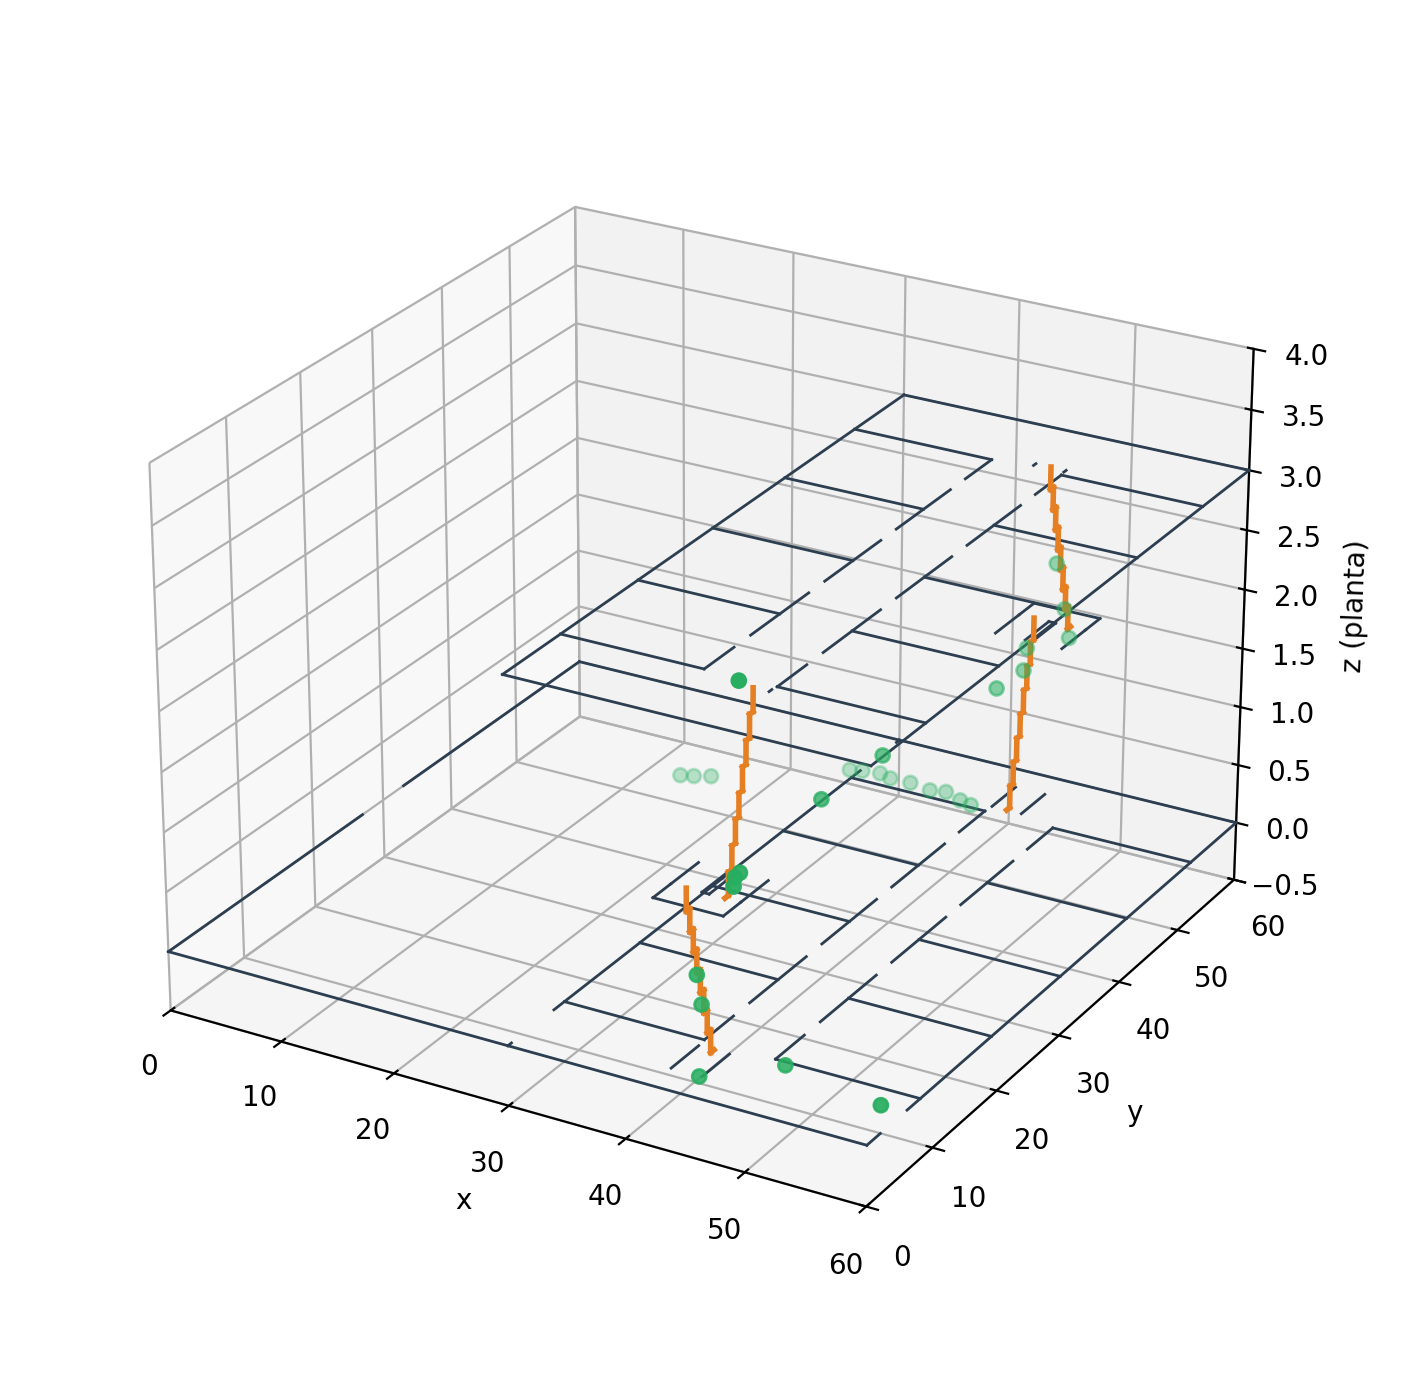
\includegraphics[width=0.78\textwidth]{escuela_3d.png}
\caption{Vista 3D apilada de la Escuela, en un instante posterior al timbre del escenario base:
los alumnos de la planta alta bajan por las dos escaleras \emph{switchback} (peldaños en
naranja). Se ven las tres capas (planta baja $z=0$, descanso $z=\SI{1.5}{\metre}$ y planta alta
$z=\SI{3}{\metre}$) con agentes distribuidos en ellas.}
\label{fig:escuela3d}
\end{figure}

\subsection*{Parámetros físicos}

El perfil físico de los agentes es el conjunto de Baglietto y Parisi~\cite{baglietto2011}. En el
sub-escenario de Evacuación los agentes usan el \emph{modo crisis}: una velocidad deseada de
emergencia $v_d = v_e = \SI{2.0}{\metre\per\second}$ (frente a los \SI{1.55}{\metre\per\second}
de la caminata normal), del orden de las velocidades deseadas usadas en modelos de escape
\cite{helbing2000}. Los parámetros de la simulación se resumen en la Tabla~\ref{tab:params}. El
paso de integración efectivo es
$\Delta t = \min\!\bigl(\Delta t_{\text{esc}},\, r_{\min}/(2\max(v_d,v_e))\bigr)$: el modelo
acota el $\Delta t$ del escenario a un valor estable para el perfil más rápido presente,
resultando $\Delta t \approx \SI{0.048}{\second}$ en caminata normal y
$\Delta t = \SI{0.0375}{\second}$ en la evacuación. La salida se registra cada
$\Delta t_{\text{out}}=\SI{0.2}{\second}$.

\begin{table}[H]
\centering
\small
\begin{tabular}{@{}lll@{}}
\toprule
\textbf{Parámetro} & \textbf{Símbolo} & \textbf{Valor} \\
\midrule
Velocidad deseada (normal)       & $v_d$   & \SI{1.55}{\metre\per\second} \\
Velocidad deseada (evacuación)   & $v_d$   & \SI{2.0}{\metre\per\second} \\
Tiempo de relajación     & $\tau$       & \SI{0.5}{\second} \\
Radio mínimo             & $r_{\min}$   & \SI{0.15}{\metre} \\
Radio máximo             & $r_{\max}$   & \SI{0.32}{\metre} \\
Coeficiente anisotrópico & $\beta$      & $0.9$ \\
Velocidad de escape      & $v_e$        & $= v_d$ \\
Paso de integración      & $\Delta t$   & \SI{0.048}{\second} / \SI{0.0375}{\second} (evac.) \\
Paso de salida           & $\Delta t_{\text{out}}$ & \SI{0.2}{\second} \\
Factor de velocidad en escalera & \texttt{speed\_factor} & $0.38$ \\
Ancho de escalera        & --           & \SI{2.6}{\metre} \\
\bottomrule
\end{tabular}
\caption{Parámetros del CPM y de la simulación. El radio máximo de cada agente se muestrea
uniforme en $[\SI{0.30}{\metre},\, \SI{0.32}{\metre}]$; la velocidad deseada de evacuación
corresponde al modo crisis (perfil por generador).}
\label{tab:params}
\end{table}

\subsection*{Barridos}

\begin{description}
  \item[Evacuación.] Los alumnos arrancan dentro de las aulas de ambas plantas y evacúan a las
  salidas; los de la planta alta bajan por las escaleras. Evacúan en \emph{modo crisis}
  ($v_d=\SI{2.0}{\metre\per\second}$). El input es la capacidad total $N$, con barrido
  $N\in\{40,80,120\}$. El tiempo total de simulación es \SI{400}{\second}.
  \item[Ingreso.] Los $N_{\max}=120$ alumnos llegan por las entradas y se dirigen a sus aulas;
  los que entran por el recreo pasan antes por el kiosco. El input es la ventana de llegada
  $T_a\in\{1,5,10\}$~min a $N_{\max}$ fijo, equivalente a un caudal
  $Q=N_{\max}/T_a\in\{120,24,12\}$ agentes/min (ec.~\ref{eq:caudal}). El tiempo total es
  $T_a + \SI{250}{\second}$.
  \item[Estudio complementario.] Sobre el mismo sub-escenario de Ingreso se varía $N_{\max}\in
  \{60,120,180\}$ a ventana fija $T_a=\SI{5}{\minute}$, para ver cómo escala la congestión con
  la cantidad de gente.
\end{description}

\paragraph{Zona de interés del Ingreso.}
El enunciado sugiere observar ``una zona, por ejemplo antes de la escalera''. Se probó el pie de
la escalera principal y no muestra congestión apreciable: la escalera \emph{switchback} es ancha
(dos carriles) y sólo la mitad de los alumnos suben a la planta alta, repartidos entre las dos
escaleras y a lo largo de la ventana, de modo que el pie queda casi vacío. La congestión del
Ingreso se forma en cambio en el frente del kiosco, donde se agolpan los alumnos que entran por
el recreo. Se adoptó como zona observable el rectángulo del kiosco, $R=[2,14]\times[42,52]$ en
$z=0$; el ``por ejemplo'' del enunciado habilita medir donde efectivamente hay congestión.

\paragraph{Realizaciones.}
Cada punto de los barridos se obtiene de \textbf{5 realizaciones} (semillas 1 a 5). Los valores
reportados son la media entre realizaciones, y las barras o el término $\pm\sigma$ indican el
desvío estándar muestral entre ellas. El criterio de evacuado es el de la ecuación~\ref{eq:tevac}.

\section{Resultados}
\label{sec:resultados}

\subsection{Evacuación}
\label{sec:evac}

La distribución de tiempos de evacuación (ec.~\ref{eq:tevac}) para las tres capacidades se
muestra en la Figura~\ref{fig:evac-hist}, y el escalar (promedio y máximo) en función de $N$ en
la Figura~\ref{fig:evac-scalar}. La Tabla~\ref{tab:evac} resume los valores.

\begin{figure}[H]
\centering
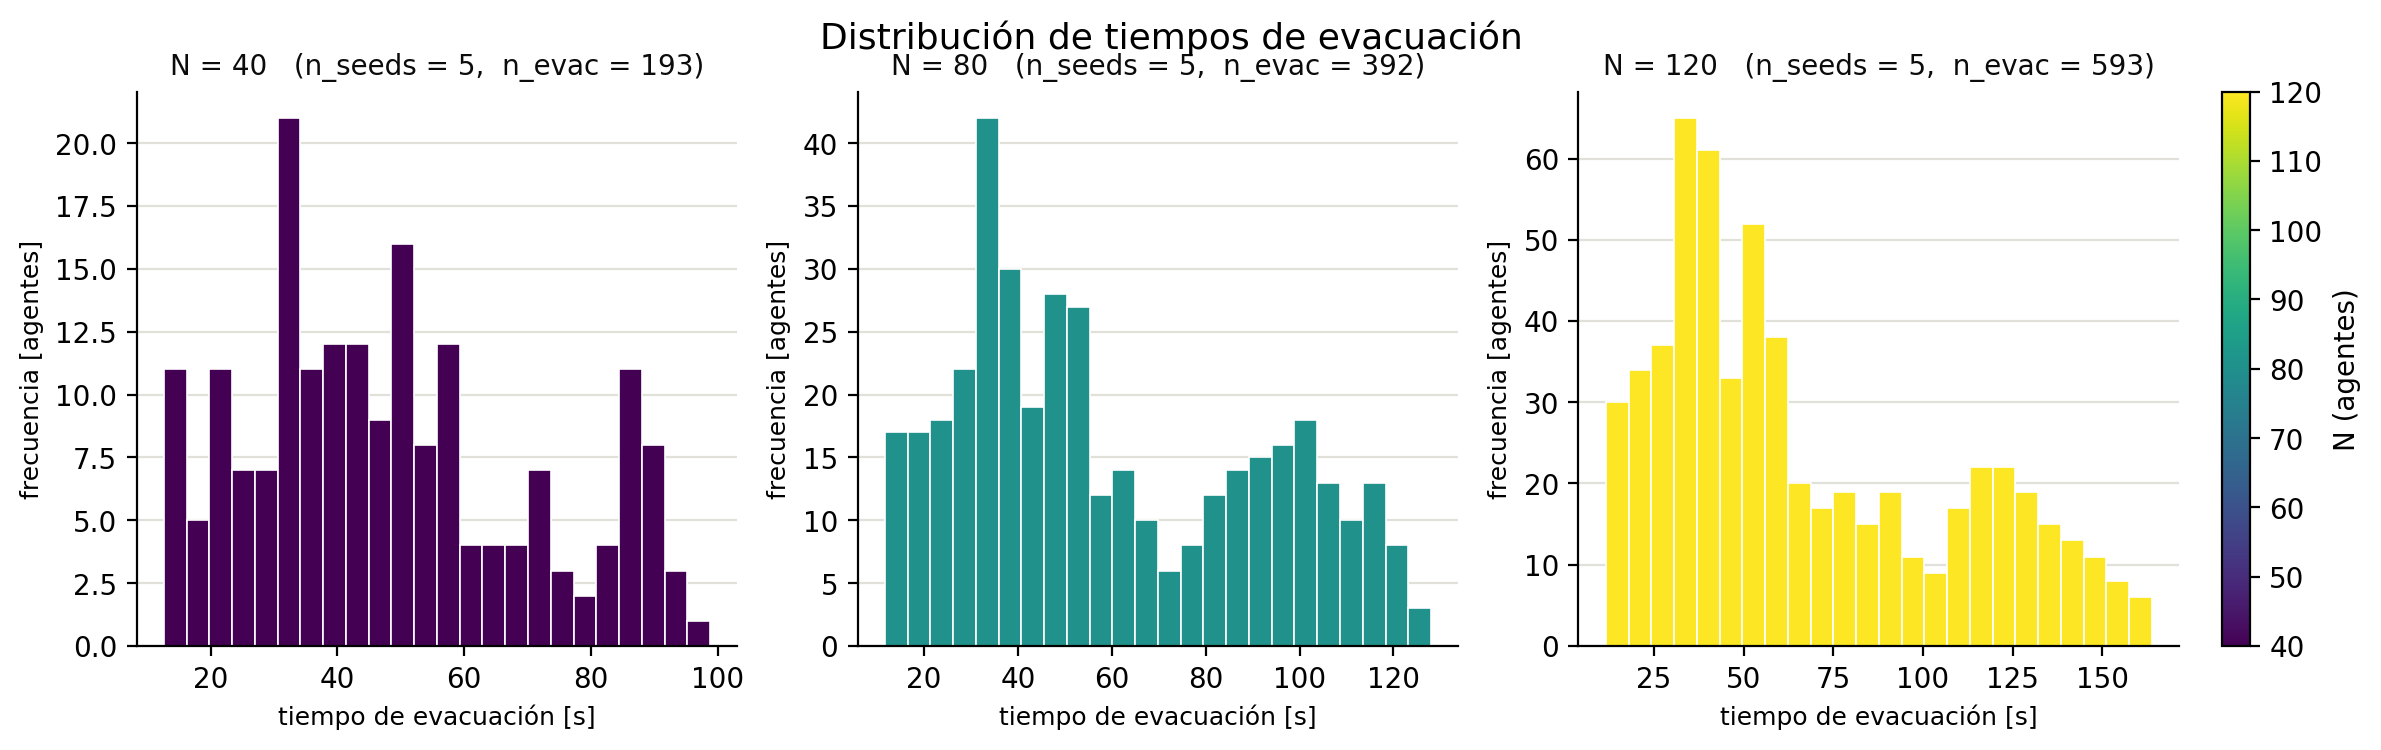
\includegraphics[width=\textwidth]{evac_hist.png}
\caption{Distribución de tiempos de evacuación para $N=40$, $80$ y $120$.}
\label{fig:evac-hist}
\end{figure}

\begin{figure}[H]
\centering
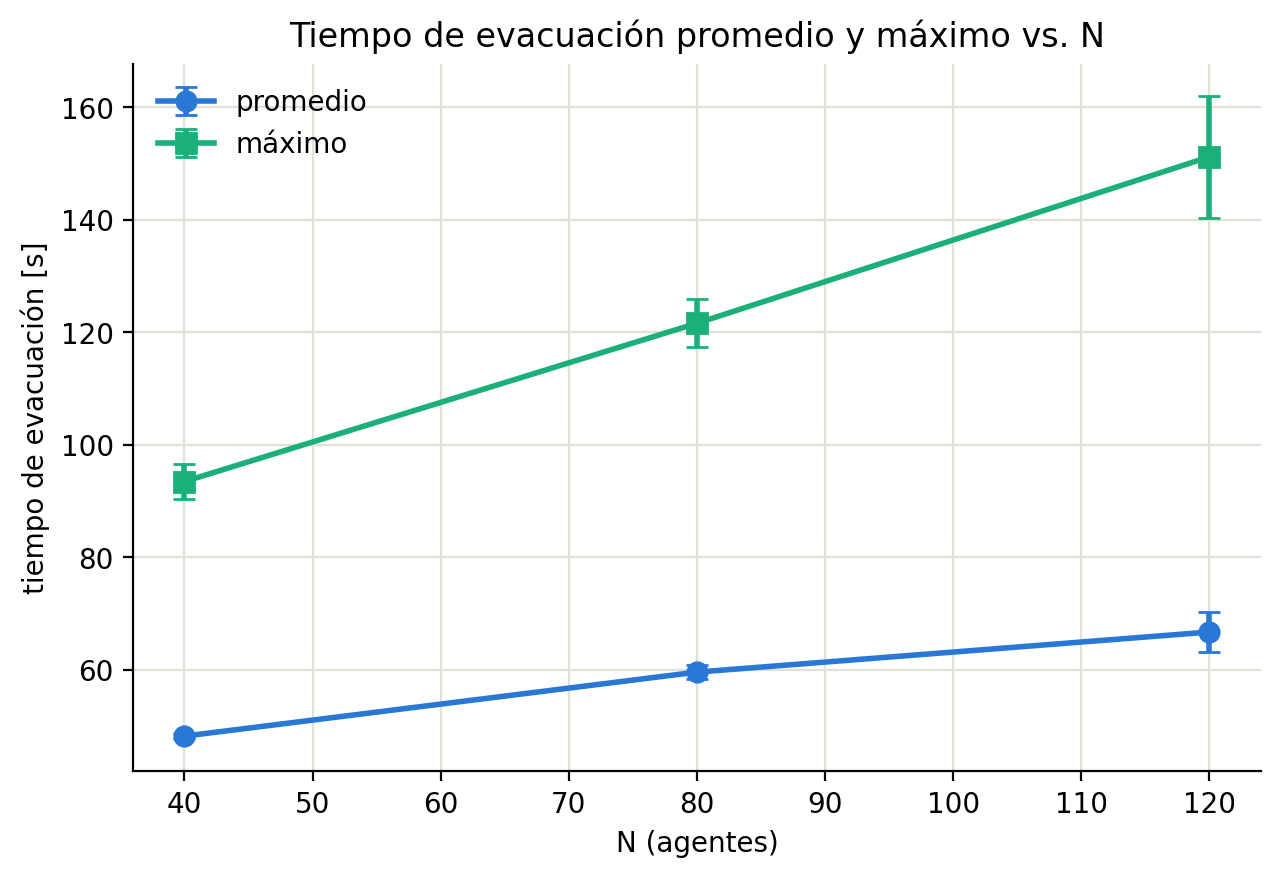
\includegraphics[width=0.62\textwidth]{evac_scalar.png}
\caption{Tiempo de evacuación promedio y máximo en función de la capacidad $N$.}
\label{fig:evac-scalar}
\end{figure}

\begin{table}[H]
\centering
\small
\begin{tabular}{@{}rrll@{}}
\toprule
$N$ & evacuados & $t_{\text{evac}}$ promedio [\si{\second}] & $t_{\text{evac}}$ máximo [\si{\second}] \\
\midrule
40  & $38.6$  & $48.2 \pm 0.6$ & $93.5 \pm 3.2$ \\
80  & $78.4$  & $59.6 \pm 1.2$ & $121.6 \pm 4.2$ \\
120 & $118.6$ & $66.7 \pm 3.6$ & $151.2 \pm 10.8$ \\
\bottomrule
\end{tabular}
\caption{Evacuación en modo crisis: agentes evacuados (media entre realizaciones), tiempo
promedio y máximo por capacidad. Cada valor es media $\pm$ desvío estándar muestral entre las
5 realizaciones.}
\label{tab:evac}
\end{table}

El tiempo de evacuación crece con $N$: al triplicar la capacidad el promedio pasa de
$48.2\pm0.6$ a $66.7\pm3.6$~\si{\second} y el máximo de $93.5\pm3.2$ a
$151.2\pm10.8$~\si{\second}. La dispersión entre realizaciones también crece con $N$ (más
congestión, más sensibilidad a la realización). La distribución es \textbf{bimodal}: un primer
lóbulo corto corresponde a los agentes de la planta baja y un segundo lóbulo lento a los de la
planta alta, que deben bajar la escalera \emph{switchback} (más larga y a velocidad reducida que
un tramo recto); el segundo lóbulo se desplaza hacia tiempos mayores al crecer $N$ y produce la
cola larga.

De los $N$ agentes no evacúan todos: queda sin evacuar $\approx 1.4$ por corrida en promedio.
Estos agentes rezagados están asociados al \emph{livelock} de jamba de puerta documentado en
\texttt{DECISIONES.md} (D14): un agente cuya dirección deseada queda casi paralela a la pared
del pasillo puede oscilar en la jamba sin cruzar. No es congestión de la escalera; se trata de
un caso residual del modelo de fuerzas mitigado con puertas más anchas.

\subsection{Ingreso}
\label{sec:ingreso}

La población en la zona del kiosco (ec.~\ref{eq:nzona}) en función del tiempo, para las tres
ventanas de llegada, se muestra en la Figura~\ref{fig:ingreso-pob}; el escalar (ocupación máxima
y promedio) en función de $T_a$ en la Figura~\ref{fig:ingreso-scalar}. La Tabla~\ref{tab:ingreso}
resume los valores.

\begin{figure}[H]
\centering
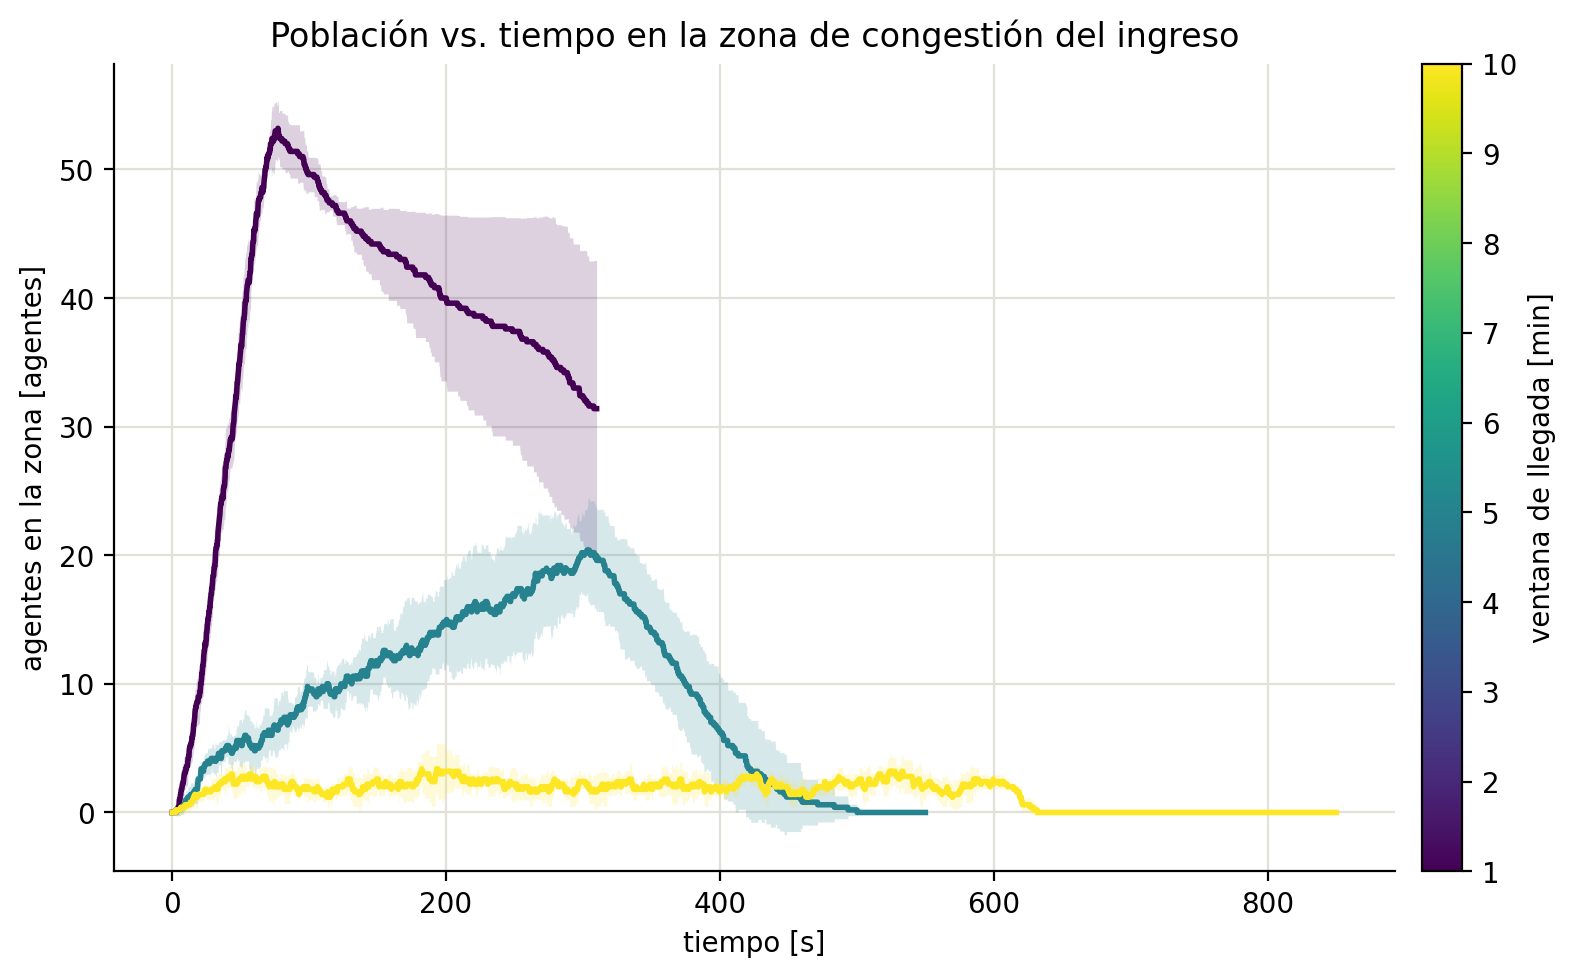
\includegraphics[width=0.85\textwidth]{ingreso_poblacion.png}
\caption{Población en la zona del kiosco vs. tiempo, para ventanas de llegada de 1, 5 y
10~minutos.}
\label{fig:ingreso-pob}
\end{figure}

\begin{figure}[H]
\centering
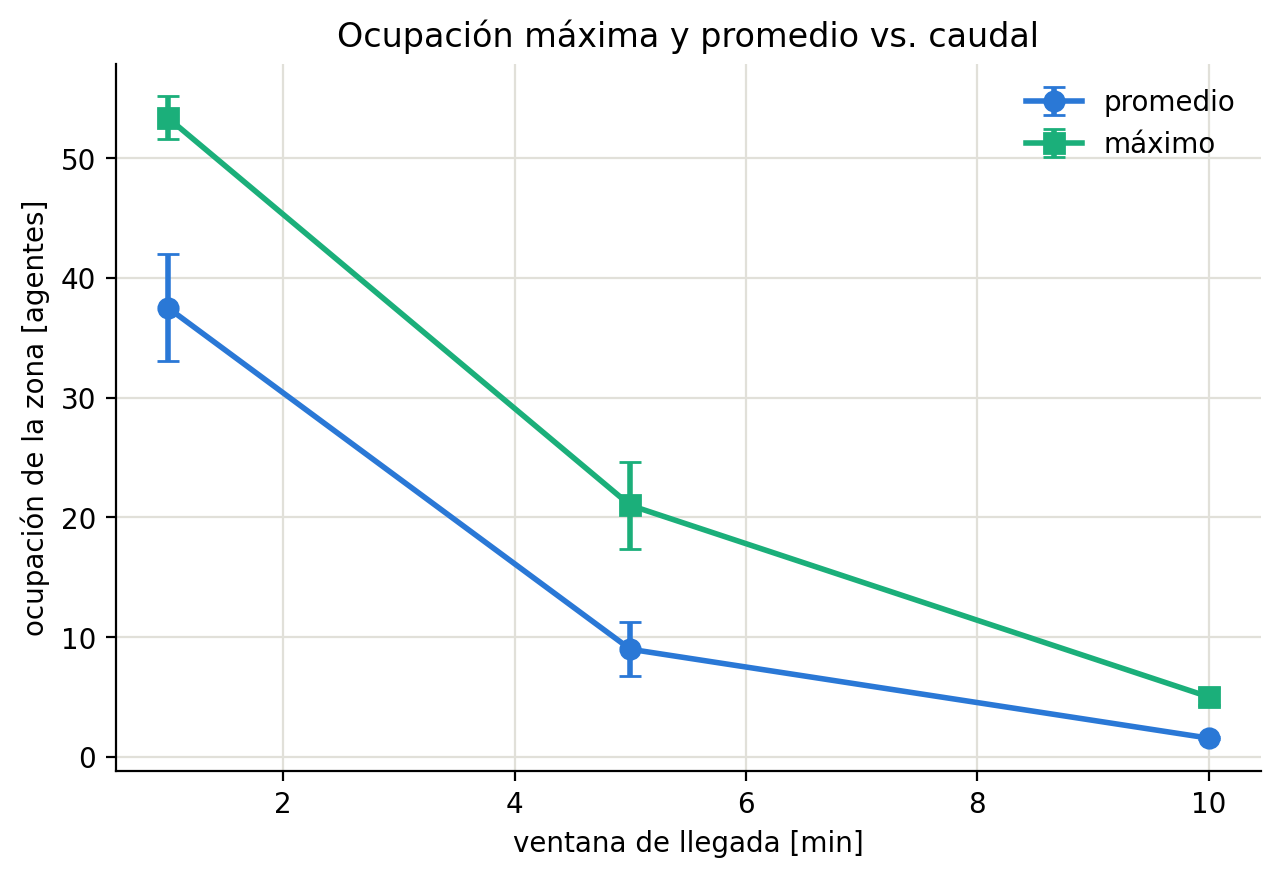
\includegraphics[width=0.62\textwidth]{ingreso_scalar.png}
\caption{Ocupación máxima y promedio de la zona en función de la ventana de llegada $T_a$.}
\label{fig:ingreso-scalar}
\end{figure}

\begin{table}[H]
\centering
\small
\begin{tabular}{@{}rrll@{}}
\toprule
$T_a$ [\si{\minute}] & $Q$ [ag./min] & Ocupación pico & Ocupación promedio \\
\midrule
1  & 120 & $53.4 \pm 1.8$ & $37.5 \pm 4.5$ \\
5  & 24  & $21.0 \pm 3.6$ & $9.0 \pm 2.3$ \\
10 & 12  & $5.0 \pm 0.7$  & $1.6 \pm 0.1$ \\
\bottomrule
\end{tabular}
\caption{Ingreso: ocupación pico y promedio en la zona del kiosco por ventana de llegada $T_a$
(caudal $Q=N_{\max}/T_a$, con $N_{\max}=120$). Valores medios entre 5 realizaciones.}
\label{tab:ingreso}
\end{table}

Con $N_{\max}$ fijo, cuanto más corta la ventana de llegada (mayor caudal $Q$), mayor la
congestión. Concentrar 120 alumnos en \SI{1}{\minute} produce un pico de $53.4\pm1.8$ agentes en
la zona, mientras que repartirlos en \SI{10}{\minute} lo baja a $5.0\pm0.7$ (una reducción de
$\sim$11$\times$). La curva de población muestra el pico agudo y temprano de la ventana de
\SI{1}{\minute} frente a la meseta baja y extendida de la de \SI{10}{\minute}: el mismo total de
personas, distinta intensidad de aglomeración. Para la ventana de \SI{1}{\minute} la cola del
kiosco no llega a drenarse dentro de la corrida ($\sim$31 agentes siguen en la zona al final):
el servidor queda saturado, otra manifestación de la misma congestión.

\subsection{Estudio complementario: cantidad de agentes}
\label{sec:nmax}

Variando $N_{\max}$ a ventana fija ($T_a=\SI{5}{\minute}$) se obtiene un eje ortogonal al del
caudal. La población en la zona vs. tiempo está en la Figura~\ref{fig:nmax-pob}, el escalar en la
Figura~\ref{fig:nmax-scalar} y los valores en la Tabla~\ref{tab:nmax}.

\begin{figure}[H]
\centering
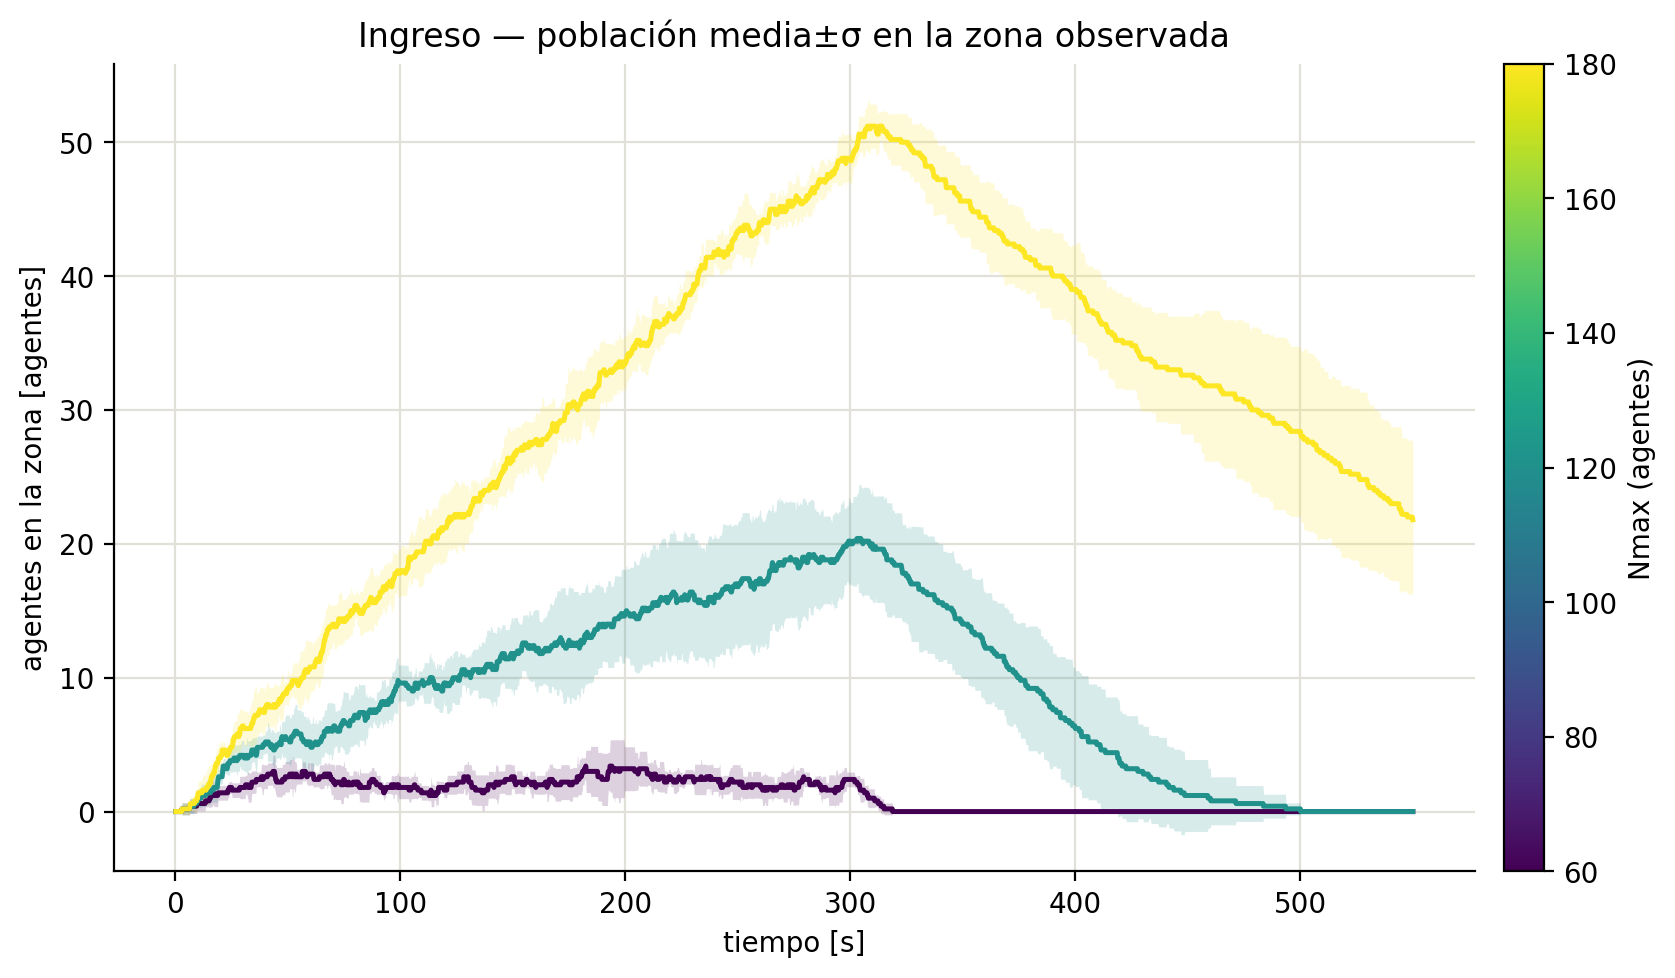
\includegraphics[width=0.85\textwidth]{ingreso_nmax_poblacion.png}
\caption{Población en la zona vs. tiempo para $N_{\max}=60$, $120$ y $180$ (ventana de
5~minutos).}
\label{fig:nmax-pob}
\end{figure}

\begin{figure}[H]
\centering
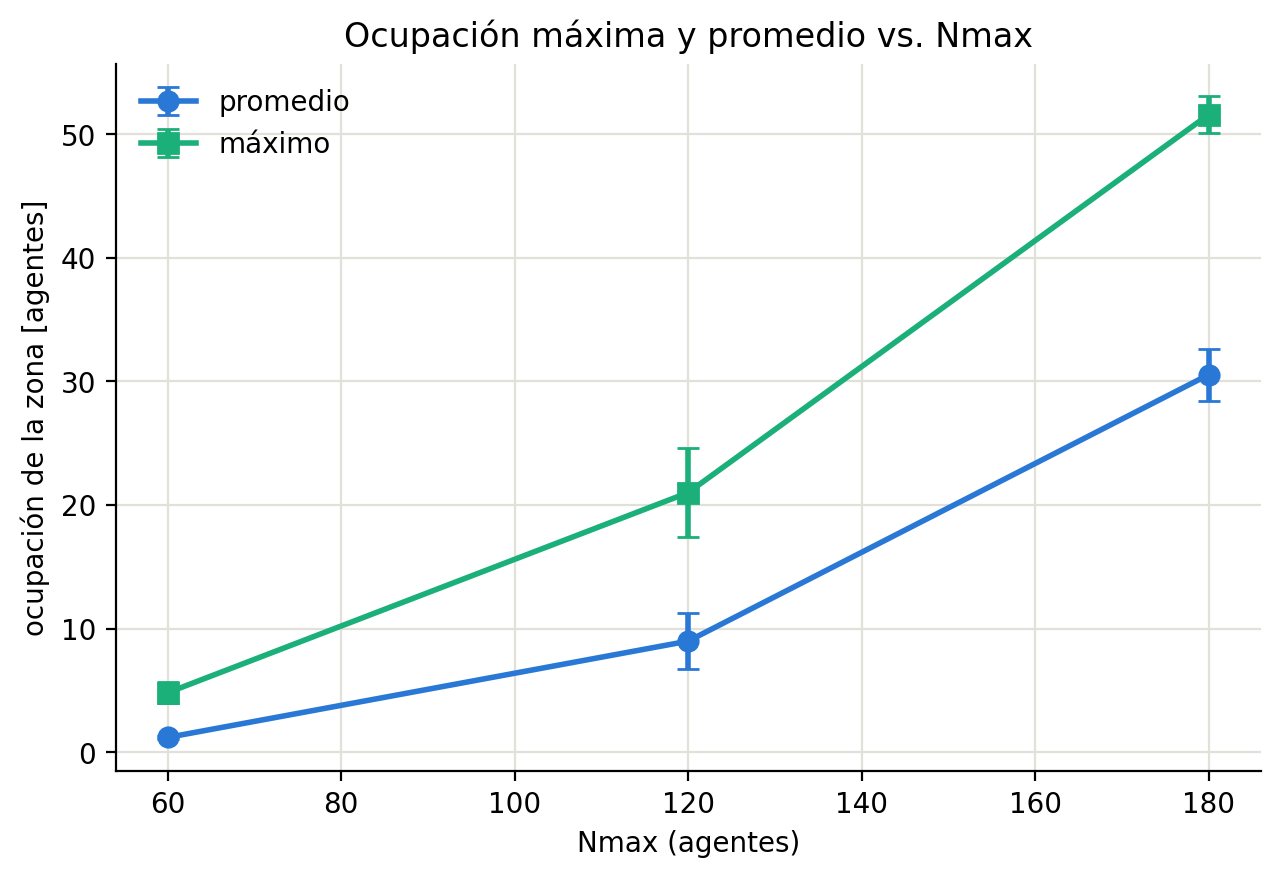
\includegraphics[width=0.62\textwidth]{ingreso_nmax_scalar.png}
\caption{Ocupación máxima y promedio de la zona en función de $N_{\max}$.}
\label{fig:nmax-scalar}
\end{figure}

\begin{table}[H]
\centering
\small
\begin{tabular}{@{}rll@{}}
\toprule
$N_{\max}$ & Ocupación pico & Ocupación promedio \\
\midrule
60  & $4.8 \pm 0.8$  & $1.2 \pm 0.2$ \\
120 & $21.0 \pm 3.6$ & $9.0 \pm 2.3$ \\
180 & $51.6 \pm 1.5$ & $30.6 \pm 2.1$ \\
\bottomrule
\end{tabular}
\caption{Estudio complementario: ocupación pico y promedio en la zona del kiosco en función de
$N_{\max}$, con ventana fija de 5~minutos. Valores medios entre 5 realizaciones.}
\label{tab:nmax}
\end{table}

La ocupación crece más que proporcionalmente con $N_{\max}$ en el rango explorado: al triplicar
la población el pico se multiplica por $\sim$11 ($4.8$, $21.0$ y $51.6$). La zona no absorbe el
flujo de forma proporcional, sino que se satura a medida que crece la cantidad de agentes.

\subsection{Mapas de calor}
\label{sec:heatmaps}

Como observable complementario se agregaron mapas de calor por planta, con colormaps
secuenciales de un solo tono y las paredes superpuestas; las celdas nunca ocupadas quedan en
gris.

\paragraph{Densidad de ocupación.}
Para cada celda de una grilla de \SI{1}{\metre}$\times$\SI{1}{\metre} se cuenta la ocupación
media (agentes dentro de la celda promediados sobre todos los cuadros de la salida). En la
evacuación (Figura~\ref{fig:dens-evac}) los puntos calientes son el pasillo central y los pies de
las escaleras, por donde todos convergen para bajar, más las dos rutas hacia las salidas. En el
ingreso (Figura~\ref{fig:dens-ing}) el punto caliente es la cola del kiosco, con los pasillos y
entradas mucho más tenues.

\begin{figure}[H]
\centering
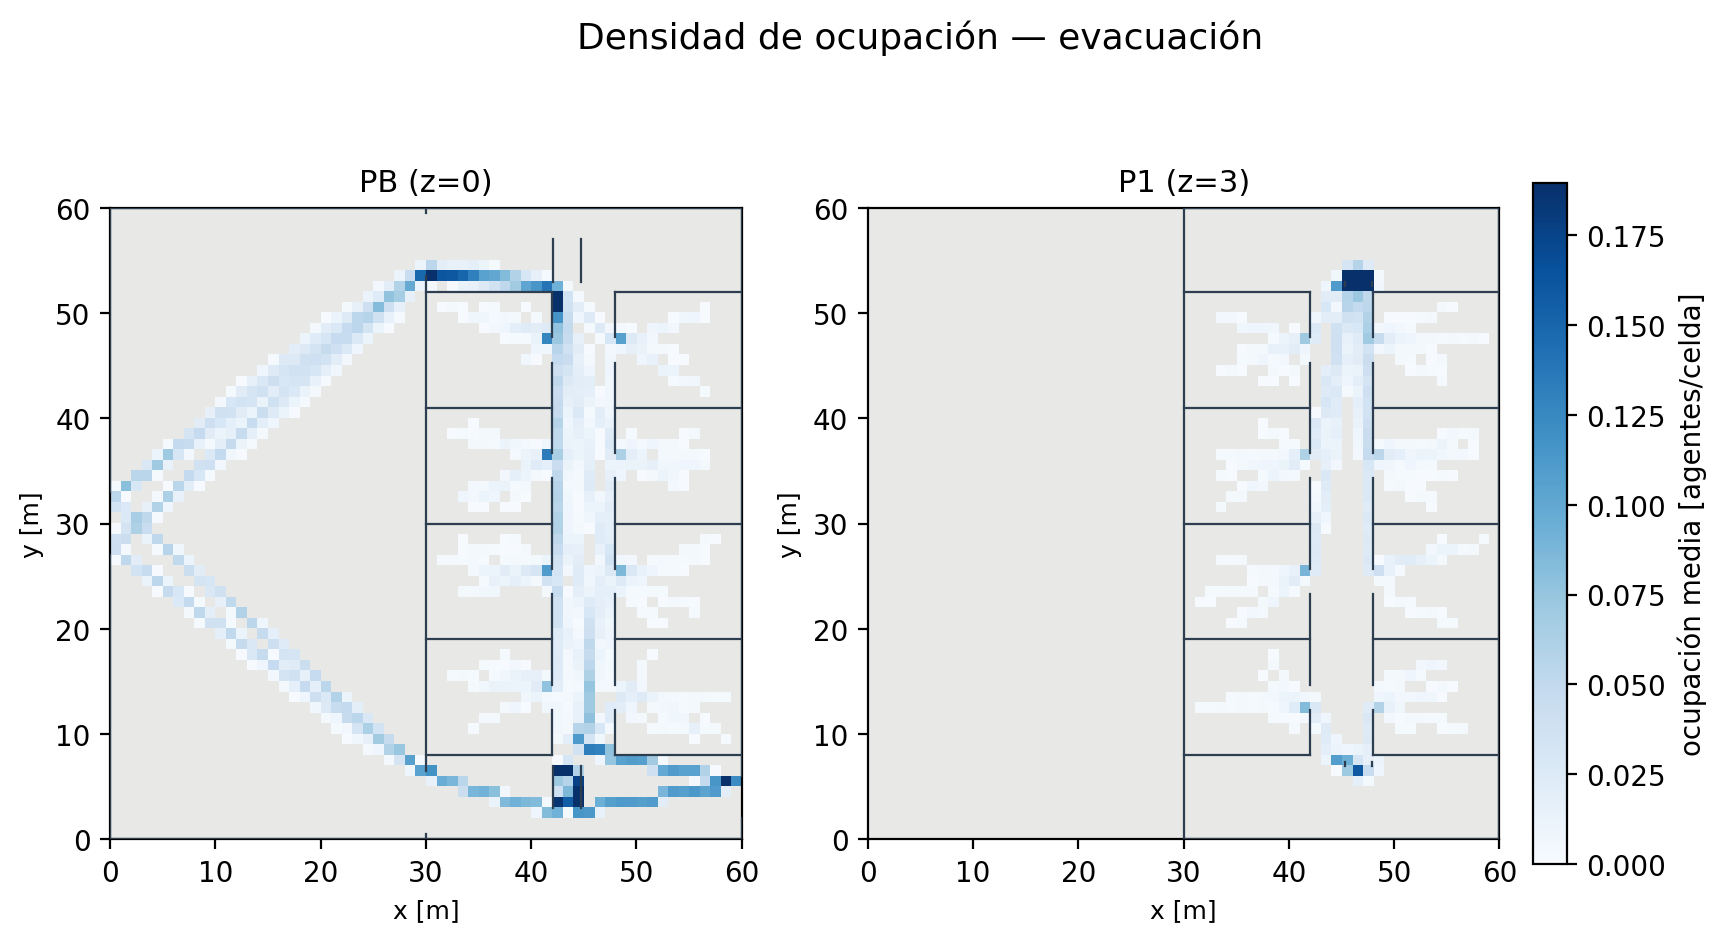
\includegraphics[width=0.86\textwidth]{heatmap_densidad_evac.png}
\caption{Densidad de ocupación durante la evacuación ($N=120$): el pasillo central y las
escaleras concentran el flujo.}
\label{fig:dens-evac}
\end{figure}

\begin{figure}[H]
\centering
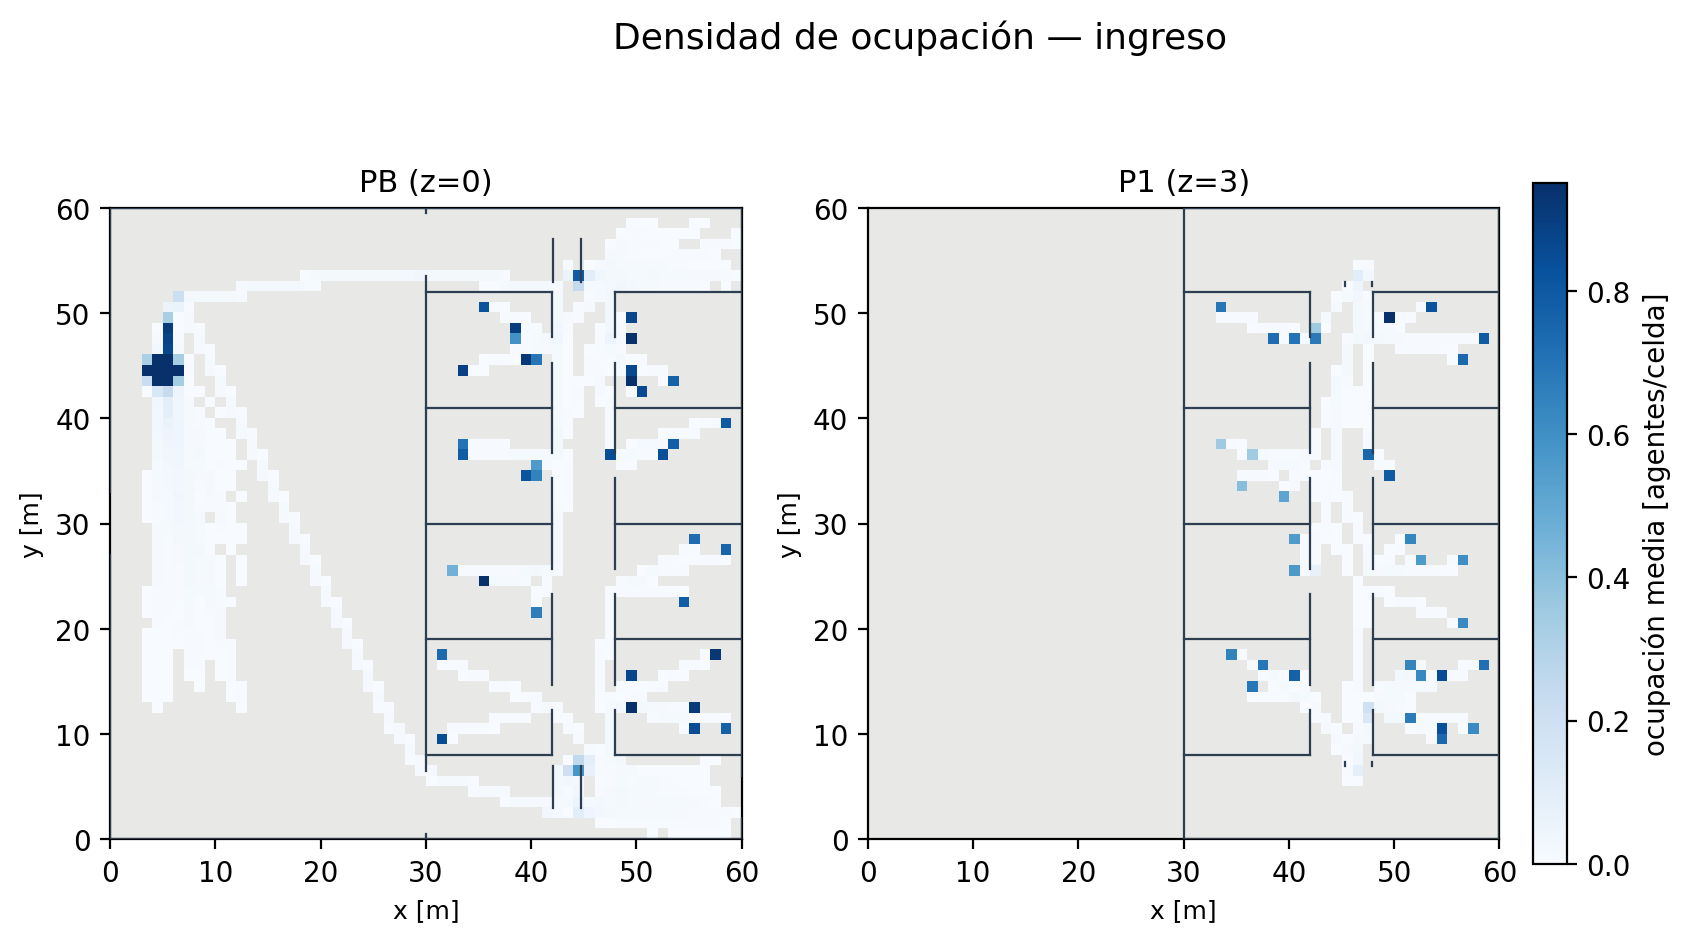
\includegraphics[width=0.86\textwidth]{heatmap_densidad_ingreso.png}
\caption{Densidad de ocupación durante el ingreso (ventana de \SI{1}{\minute}): la cola del
kiosco es el punto caliente.}
\label{fig:dens-ing}
\end{figure}

\paragraph{Tiempos de evacuación por origen.}
Se toma el punto de origen de cada agente (su primer cuadro) y se colorea la celda con el tiempo
de evacuación medio de los agentes que arrancan ahí (Figura~\ref{fig:tevac}). Las aulas de la
planta baja evacúan en $\sim$15--\SI{60}{\second} (mediana \SI{36}{\second}), mientras que las de
la planta alta tardan $\sim$60--\SI{140}{\second} (mediana \SI{95}{\second}), porque deben bajar
la escalera. El mapa cuantifica espacialmente el costo de estar en la planta alta.

\begin{figure}[H]
\centering
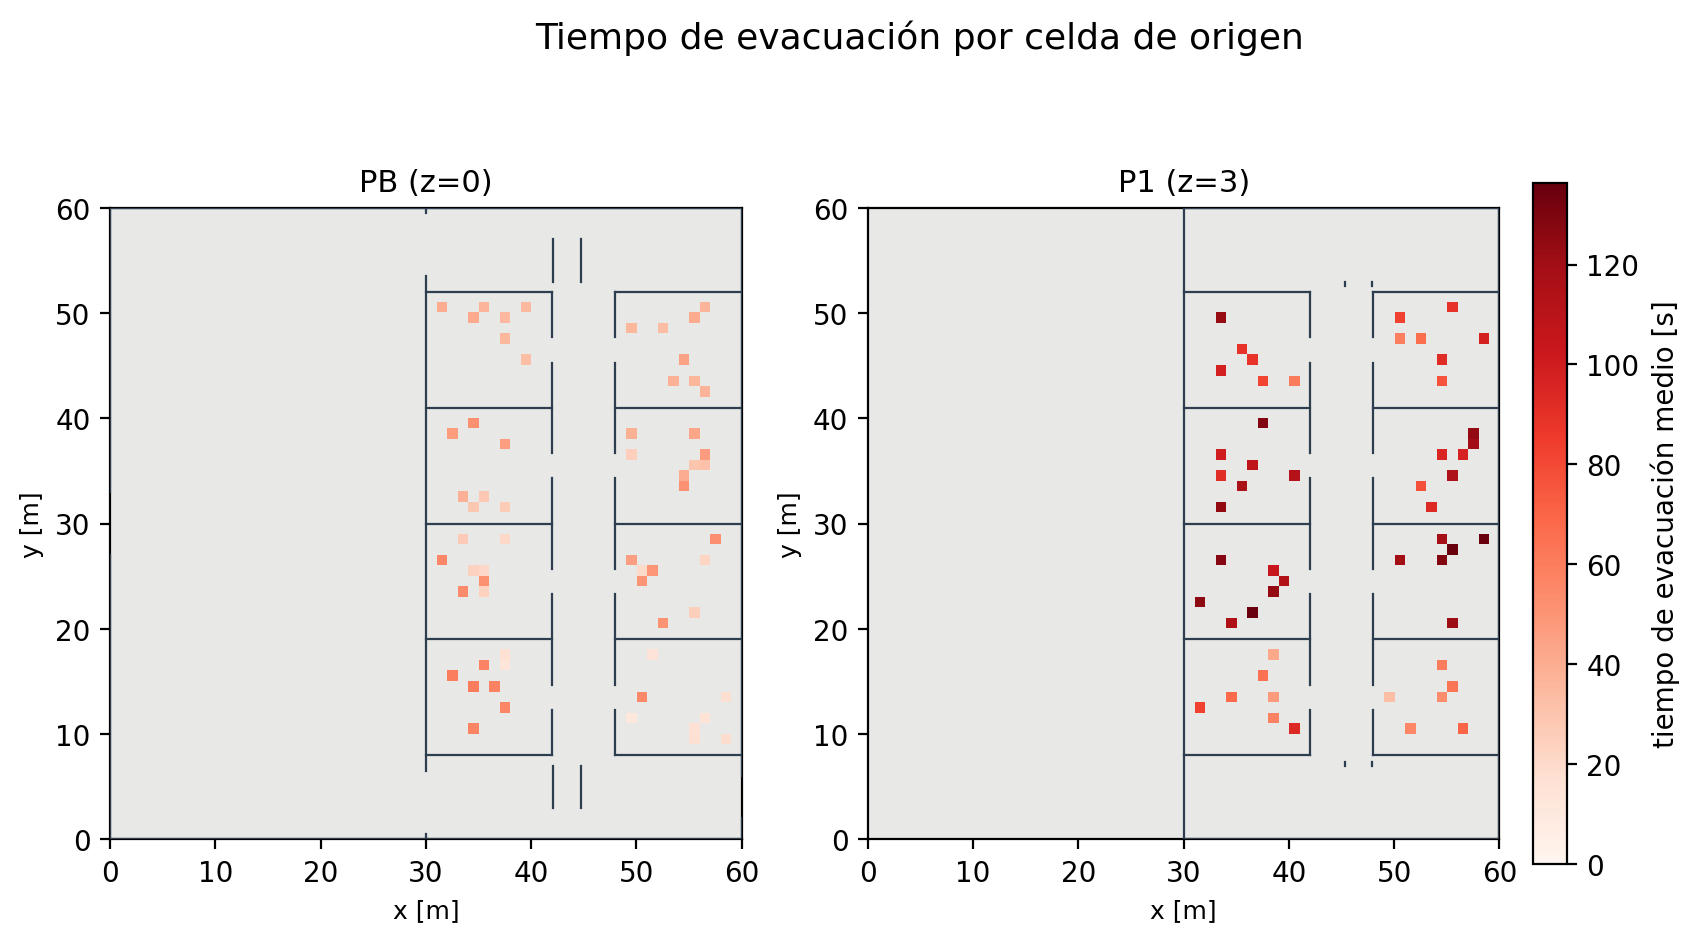
\includegraphics[width=0.86\textwidth]{heatmap_tevac.png}
\caption{Tiempo de evacuación medio según la celda de origen ($N=120$). Las aulas de la planta
alta (tonos oscuros) evacúan mucho más lento que las de la planta baja por tener que descender
por las escaleras.}
\label{fig:tevac}
\end{figure}

\section{Conclusiones}
\label{sec:conclusiones}

\begin{itemize}
  \item El simulador quedó ampliado a 3D de punta a punta: agentes con $z\neq 0$ que recorren
  escaleras a velocidad reducida, detección de vecinos y física por planta, grafo de navegación
  3D (A* euclídeo unido por escaleras), salida con $z$ y animación 2D por planta más vista 3D
  apilada.
  \item La escalera \emph{switchback} con descanso, confinamiento y carriles de contraflujo da
  un comportamiento coherente; el artefacto del salto de $z$ se diagnosticó y resolvió.
  \item En la evacuación, el tiempo de evacuación crece con la capacidad $N$ (promedio y máximo)
  en el rango explorado, y su distribución es bimodal: los agentes de la planta baja salen
  rápido y los de la planta alta forman el lóbulo lento, que se corre a tiempos mayores al
  crecer $N$.
  \item En el ingreso, la ocupación de la zona observada crece al acortar la ventana de llegada
  (mayor caudal) y, en el estudio complementario, crece más que proporcionalmente con $N_{\max}$.
  \item En promedio $1.4$ agentes por corrida no evacúan, por el \emph{livelock} de jamba de
  puerta del modelo de fuerzas; es un límite conocido, mitigado pero no eliminado.
\end{itemize}

\begin{thebibliography}{9}
\bibitem{baglietto2011}
G.~Baglietto y D.~R.~Parisi,
\emph{Continuous-space automaton model for pedestrian dynamics},
Physical Review E \textbf{83}, 056117 (2011).
% Referencia canónica del CPM ("Baglietto & Parisi"), citada en CpmParameters.java.

\bibitem{martin2024}
R.~Martin y D.~R.~Parisi,
\emph{Anisotropic Contractile Particle Model with Avoidance (A-CPM)}, 2024.
% Variante anisotrópica con evitación usada en el código
% (CpmOperationalModel.java: "based on Martin & Parisi (2024)", §3.2).

\bibitem{helbing2000}
D.~Helbing, I.~Farkas y T.~Vicsek,
\emph{Simulating dynamical features of escape panic},
Nature \textbf{407}, 487--490 (2000).
% Referencia clásica de dinámica de escape: velocidades deseadas elevadas en crisis.
\end{thebibliography}

\appendix
\section{Reproducción de los resultados}
\label{sec:reproduccion}

\begin{lstlisting}[language=bash]
# Compilar y tests
mvn clean test                      # 143 tests, 0 fallos, 0 omitidos

# Escenario Escuela (baseline) + animacion 3D
python tools/scenarios-builders/build_escuela.py
mvn -q dependency:build-classpath -Dmdep.outputFile=out/.cp.txt
java -Dsimped.seed=1 -cp "target/classes:$(cat out/.cp.txt)" \
     ar.edu.itba.simped.App scenarios/escuela out/escuela.csv cpm
python tools/visualize_simulation_3d.py --scenario scenarios/escuela \
     --output out/escuela.csv --out out/escuela_3d.mp4 --stride 3

# Evacuacion: barrido N en {40, 80, 120}, 5 semillas + figuras
python tools/sweep_run.py --mode evacuacion --values 40,80,120 --seeds 1,2,3,4,5 --om cpm
python tools/plot_evacuacion.py --sweep-dir out/sweeps/evacuacion --seeds all --out-prefix out/evac

# Ingreso: barrido caudal 1/5/10 min, 5 semillas + figuras
python tools/sweep_run.py --mode ingreso --values 1,5,10 --seeds 1,2,3,4,5 --om cpm
python tools/plot_ingreso.py --sweep-dir out/sweeps/ingreso --seeds all --out-prefix out/ingreso

# Ingreso variando la cantidad de agentes (estudio complementario)
python tools/run_ingreso_nmax.py --nmax 60,120,180 --window 5 --seeds 1,2,3,4,5
\end{lstlisting}

\end{document}
